\subsection{Question 1}

\lstinputlisting[caption=Matlab Commands,showstringspaces=false,language=Matlab]{../find_vectors.m}

\newpage
\subsubsection{Part A}

\lstinputlisting[caption=Matlab Commands,showstringspaces=false,language=Matlab]{../q1_partA}

\subsubsection{Part B}

\lstinputlisting[caption=Matlab Commands,showstringspaces=false,language=Matlab]{../q1_partB}

\newpage
\subsection{Question 2}

\begin{figure}[th]
  \centering
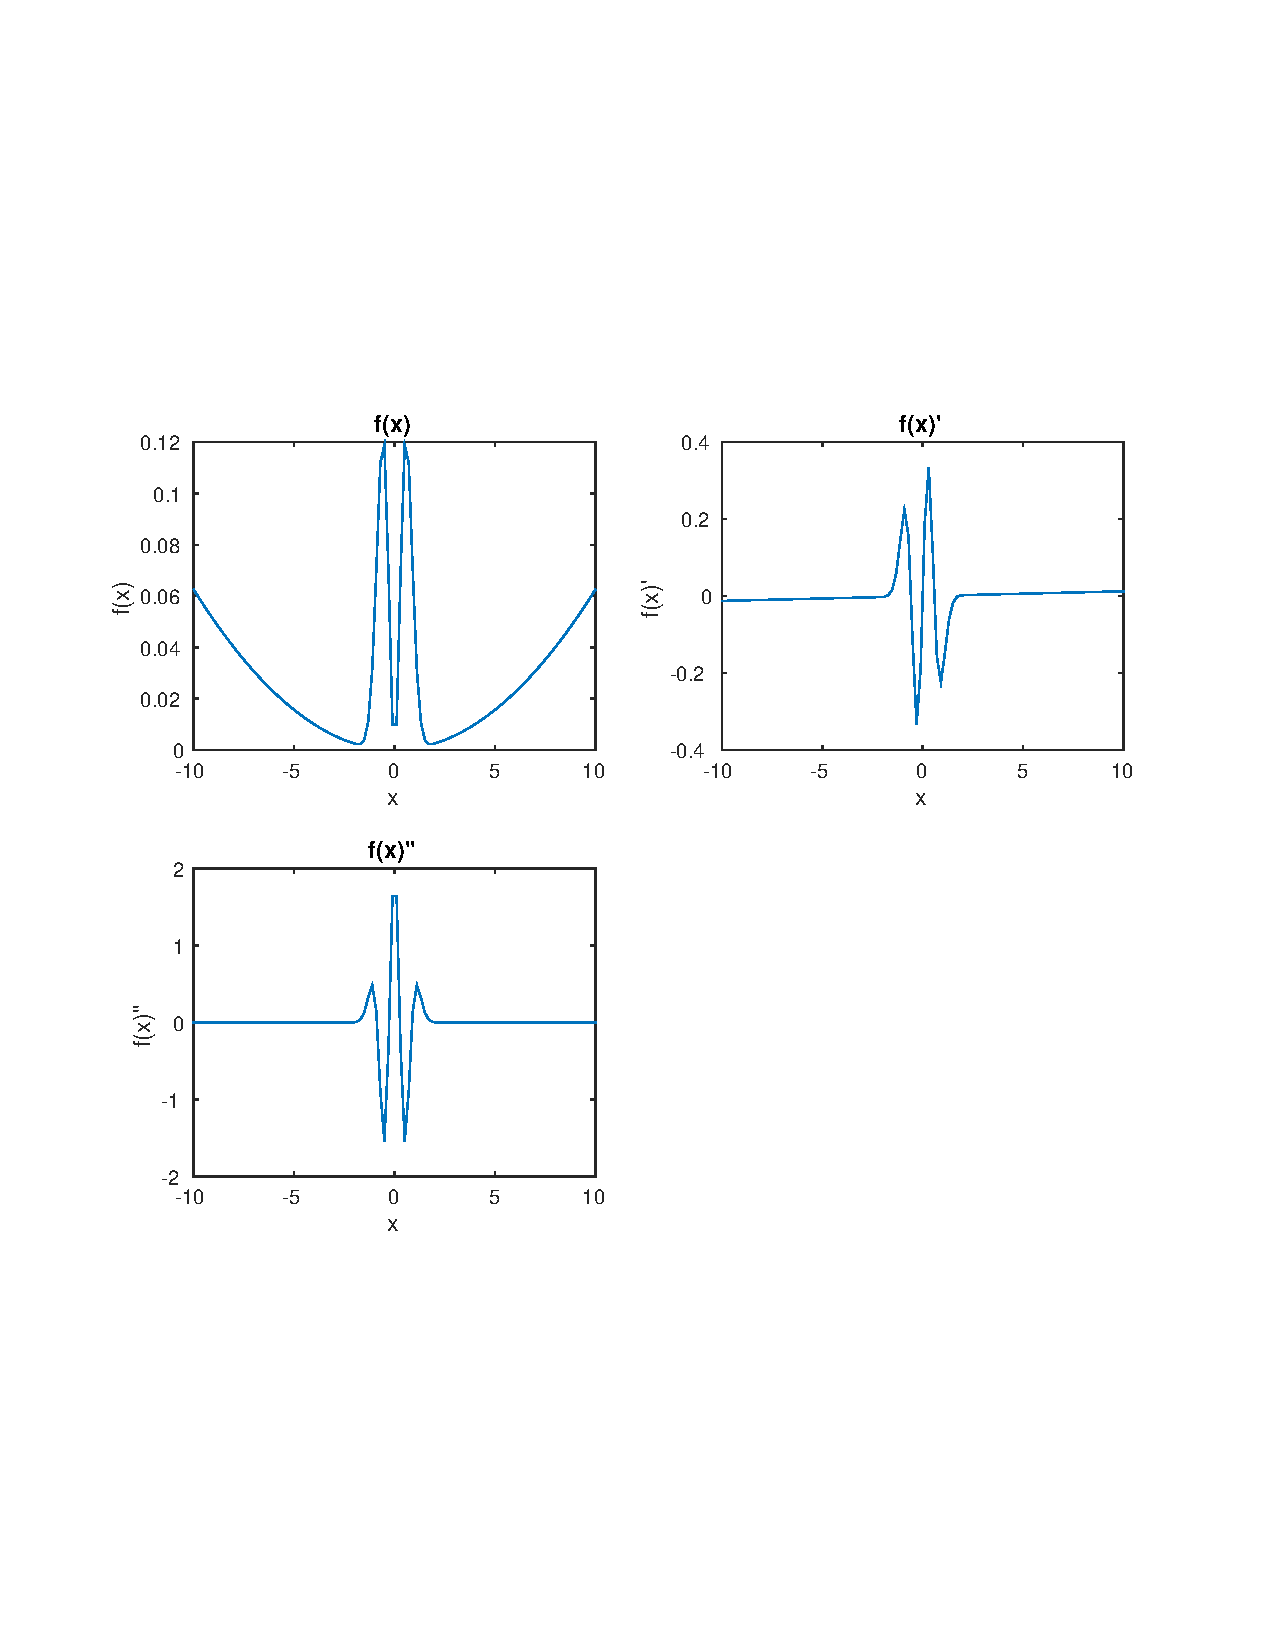
\includegraphics[trim=10mm 70mm 10mm 70mm, width=1.0\textwidth]{../q2_plots}
\end{figure}

\lstinputlisting[caption=Matlab Commands,showstringspaces=false,language=Matlab]{../q2_maxmin}

\newpage
\lstinputlisting[caption=Matlab Commands,showstringspaces=false,language=Matlab]{../q2_plots}

\newpage
\subsection{Question 3}

\subsubsection{Part C}

The claim made from assignment 2 question 3 part B was as follows:

\begin{eqnarray}
  ||A^{-1}||_2 = \max_{s_A \in s(A)} \{\frac{1}{s_a}\}
\end{eqnarray}

We must find a formula for the condition number of \(A\), \(c_2(A)\), in terms of \(\sigma(A'A)\).
Note, we know \(||A||_2 = \max \{ s(A) \}\) where \(s(A)\) are the singular values of \(A\).
The formula for the condition number of \(A\) is as follows:

\begin{eqnarray}
  c_2(A) = ||A||_2||A^{-1}||_2
  \label{form:c2}
\end{eqnarray}

Therefore, to define \(c_2(A)\) in terms of the \(\sigma(A'A)\) we simply substitute our formulas for \(||A||_2\) and \(||A^{-1}||_2\) into (\ref{form:c2}).
This yeilds,

\begin{eqnarray}
  c_2(A) = \max \{s(A)\} \max_{s_A \in s(A)} \{\frac{1}{s_a}\}
\end{eqnarray}

\subsubsection{Part D}

The claim made from assignment 2 question 2 part E was as follows:

\begin{eqnarray}
  s(A) = \{|\lambda| : \lambda \in \sigma(A), \lambda \neq 0\}
  \label{form:sasym}
\end{eqnarray}

Stated, this says ''The singular values of a matrix \(A\) are the absolute values of the non-zero eigenvalues of \(A\), where \(A\) is symmetric''.

The formula for the condition number of a symmetric matrix \(A\) is the same as the formula stated in part C.
The only change in definition is that of the singular values of \(A\).
Thefore the formula, using the definition of \(s(A)\) from \ref{form:sasym}, is,

\begin{eqnarray}
  c_2(A) &=& \max \{s(A)\} \max_{s_A \in s(A)} \{\frac{1}{s_a}\}
\end{eqnarray}

\newpage
\subsubsection{Part E}

\lstinputlisting[caption=Matlab Commands,showstringspaces=false,language=Matlab]{../q3_partE}



\newpage
\subsection{Question 4}

\subsubsection{Part A}

\lstinputlisting[caption=Matlab Commands,showstringspaces=false,language=Matlab]{../q4_partA.m}

\subsubsection{Part B}

\lstinputlisting[caption=Matlab Commands,showstringspaces=false,language=Matlab]{../q4_partB.m}

\newpage
\subsubsection{Part C}

\begin{figure}[th]
  \centering
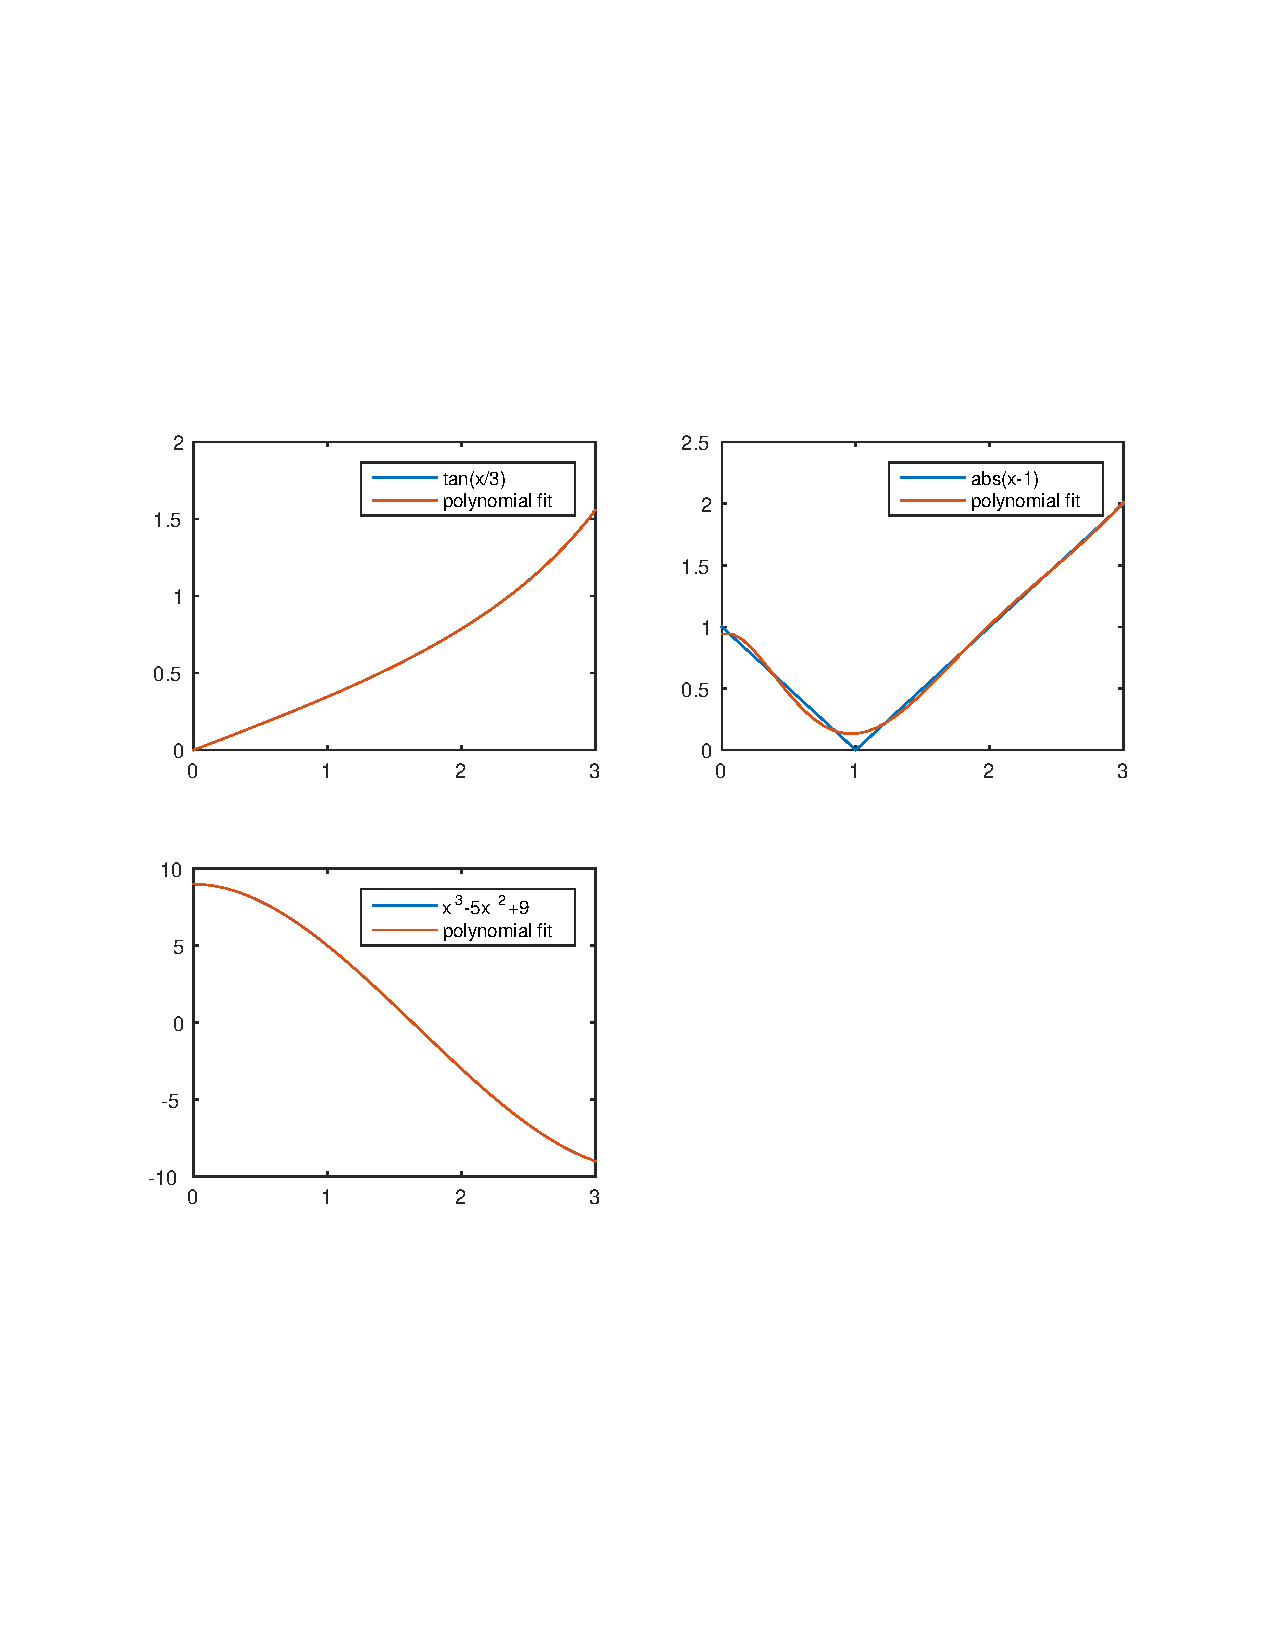
\includegraphics[trim=10mm 70mm 10mm 70mm, width=1.0\textwidth]{../q4_plots}
\end{figure}

From these plots we can see that a higher order polynomial is quite good at fitting a lower order polynomial on a small range.
This is apparent from the plots of \(\tan(\frac{x}{3})\) and \(x^{3}-5x^{2}+9\).
However, the fit is less tight for \(|x-1|\), a function that has a point where it is not differentiable (e.g., in general, non-smooth functions).

Note, the error norm is \(||p(T)-f(T)||_2\).
\lstinputlisting[caption=Matlab Commands,showstringspaces=false,language=Matlab]{../q4_partD}

\newpage
\lstinputlisting[caption=Matlab Commands,showstringspaces=false,language=Matlab]{../q4_partC}

\newpage
\subsection{Question 5}
\subsubsection{Part A}

We must prove that a matrix \(A\) with a real Cholesky factorization is symmetric positive definite.
Therefore we must prove two things.
The first is that \(A\) is positive definite.
The second is that \(A\) is symmetric.
To this end we know \(A = C'C\).

Therefore we can prove positive definiteness simply as follows,

\begin{eqnarray}
  (Av,v) &\ge& 0 \\
  (C'Cv,v) &\ge& 0 \\
  (Cv,Cv) &\ge& 0
\end{eqnarray}

This concludes the proof for positive definiteness.

Next, we will prove that \(A\) is symmetric.
Note, a matrix \(A\) is symmetric if \(A = A'\).
The proof is a simple substitution as follows,

\begin{eqnarray}
  A &=& A' \\
  C'C &=& (C'C)' \\
  C'C &=& C'C
\end{eqnarray}

This concludes the proof that \(A\) is symmetric.
The proof that \(A\) is symmetric positive definite is complete.

\subsubsection{Part B}

We must find the \(LDU\) factorization of \(A\).
To this end we will first find the \(LU\) factorization and then extract \(D\).

\begin{eqnarray}
  A =
  \begin{bmatrix}
    2 & 2 & 3 \\
    2 & 4 & 5 \\
    3 & 5 & 8
  \end{bmatrix}
\end{eqnarray}

We must find the \(L\) matrices that transform \(A\) to \(U\).

\begin{eqnarray}
  L_1 &=& 
  \begin{bmatrix}
    1 & 0 & 0 \\
    -1 & 1 & 0 \\
    -1.5 & 0 & 1 \\
  \end{bmatrix}
  \\
  A_1 &=&
  \begin{bmatrix}
    1 & 0 & 0 \\
    -1 & 1 & 0 \\
    -1.5 & 0 & 1 \\
  \end{bmatrix}
  \begin{bmatrix}
    2 & 2 & 3 \\
    2 & 4 & 5 \\
    3 & 5 & 8    
  \end{bmatrix}
  \\
  A_1 &=&
  \begin{bmatrix}
    2 & 2 & 3 \\
    0 & 2 & 2 \\
    0 & 2 & 3 \\
  \end{bmatrix}
  \\
  L_2 &=& 
  \begin{bmatrix}
    1 & 0 & 0 \\
    0 & 1 & 0 \\
    0 & -1 & 1 \\
  \end{bmatrix}
  \\
  A_2 &=&
  \begin{bmatrix}
    1 & 0 & 0 \\
    0 & 1 & 0 \\
    0 & -1 & 1 \\
  \end{bmatrix}
  \begin{bmatrix}
    2 & 2 & 3 \\
    2 & 4 & 5 \\
    3 & 5 & 8    
  \end{bmatrix}
  \\
  A_2 &=&
  \begin{bmatrix}
    2 & 2 & 3 \\
    0 & 2 & 2 \\
    0 & 0 & 1.5 \\
  \end{bmatrix}
\end{eqnarray}

Now we gather the terms from \(L_1\) and \(L_2\) (flipping signs to obtain the inverse) for our matrix \(L\).
The matrix \(U\) is simply \(A_2\).
In total,

\begin{eqnarray}
  L =
  \begin{bmatrix}
    1 & 0 & 0 \\
    1 & 1 & 0 \\
    1.5 & 1 & 1 \\
  \end{bmatrix}
  U =
  \begin{bmatrix}
    2 & 2 & 3 \\
    0 & 2 & 2 \\
    0 & 0 & 1.5 \\
  \end{bmatrix}
\end{eqnarray}

Now, we factor \(D\) from \(U\).
We simply pull out the diagonal and scale each row of \(U\) by the diagonal element of \(D\).
This changes \(U\) so we are left with,

\begin{eqnarray}
  L =
  \begin{bmatrix}
    1 & 0 & 0 \\
    1 & 1 & 0 \\
    1.5 & 1 & 1 \\
  \end{bmatrix}
  D =
  \begin{bmatrix}
    2 & 0 & 0 \\
    0 & 2 & 0 \\
    0 & 0 & 1.5 \\
  \end{bmatrix}
  U =
  \begin{bmatrix}
    1 & 1 & 1.5 \\
    0 & 1 & 1 \\
    0 & 0 & 1 \\
  \end{bmatrix}
\end{eqnarray}

\subsubsection{Part C}

The matrix \(A\) is positive definite.
This is because all the diagonal entries in \(D\) are positive which suffices to prove a matrix is positive definite.

\subsubsection{Part D}

To find a Cholesky factorization of \(A\) we will use the \(LDU\) factorization.
We will split \(D\) into two equal matrices by taking the square root's of the diagonal entries.
Therefore,

\begin{eqnarray}
  A &=&
  \underbrace{
  \begin{bmatrix}
    1 & 0 & 0 \\
    1 & 1 & 0 \\
    1.5 & 1 & 1 \\
  \end{bmatrix}
  \begin{bmatrix}
    \sqrt{2} & 0 & 0 \\
    0 & \sqrt{2} & 0 \\
    0 & 0 & \sqrt{1.5} \\
  \end{bmatrix}
  }_{\text{C'}}
  \underbrace{
  \begin{bmatrix}
    \sqrt{2} & 0 & 0 \\
    0 & \sqrt{2} & 0 \\
    0 & 0 & \sqrt{1.5} \\
  \end{bmatrix}
  \begin{bmatrix}
    1 & 1 & 1.5 \\
    0 & 1 & 1 \\
    0 & 0 & 1 \\
  \end{bmatrix}
  }_{\text{C}}
  \\
  A &=&
  \underbrace{
  \begin{bmatrix}
    1.4142 & 0 & 0 \\
    1.4142 & 1.4142 & 0 \\
    2.1213 & 1.4142 & 1.2247 \\
  \end{bmatrix}
  }_{\text{C'}}
  \underbrace{
  \begin{bmatrix}
    1.4142 & 1.4142 & 2.1213 \\
    0 & 1.4142 & 1.4142 \\
    0 & 0 & 1.2247 \\
  \end{bmatrix}
  }_{\text{C}}
\end{eqnarray}

\lstinputlisting[caption=Matlab Commands,showstringspaces=false,language=Matlab]{../q5_partD}

\newpage
\subsection{Question 6}

The matrix \(A\) is singular.
Note, this means this does not contradict the theorem that proves a solution is unique because we will solve an underdetermined system which gives us a free variable.
We can find solutions to \(Ax=b\) through the normal equations solution.
Therefore, we will solve \(A'Ax=A'b\).

\begin{eqnarray}
  A'Ax &=& A'b \\
  LUx &=& A'b \\
  Ly &=& A'b \\
  y &=& L \setminus (A'b) \\
  x &=& U \setminus x
\end{eqnarray}

\lstinputlisting[caption=Matlab Commands,showstringspaces=false,language=Matlab]{../q6}

Now we will solve,

\begin{eqnarray}
  Ux &=& y \\
  \begin{bmatrix}
    90 & 108 & 126 \\
    0 & -1.2 & -2.4 \\
    0 & 0 & 0 \\
  \end{bmatrix}
  x &=&
  \begin{bmatrix}
    12 \\
    -0.8 \\
    0 \\
  \end{bmatrix}
\end{eqnarray}

This is an underdetermined system so we set \(x_3 = c\) and solve.
This yields \(x_2 = -2c + 0.6667\) and \(x_1 = c - 0.6667\).
Now we simply choose three values for \(c\).

\begin{eqnarray}
  c = 1 \Rightarrow
  \begin{bmatrix}
     0.3333 \\
    -1.3333 \\
    1 \\
  \end{bmatrix}
  c = 2 \Rightarrow
  \begin{bmatrix}
    1.3333 \\
    -3.3333 \\
    2 \\
  \end{bmatrix}
  c = 3 \Rightarrow
  \begin{bmatrix}
    2.3333 \\
    -5.3333 \\
    3 \\
  \end{bmatrix}
\end{eqnarray}
